\documentclass[UTF8,a4paper,11pt,fontset=none]{ctexart}
\usepackage{fontspec}\setmainfont{Times New Roman}\setsansfont{Arial}\setmonofont{Menlo}\setCJKmainfont{Songti SC}\setCJKsansfont{Heiti SC}
\usepackage[margin=2.2cm]{geometry}\usepackage{amsmath,amssymb,graphicx,booktabs,tabularx,hyperref,microtype}
\hypersetup{hidelinks}
\setlength{\parskip}{.4em}\setlength{\emergencystretch}{2em}
\title{电流模式怎样影响材料反演？\\关于内部反馈、双向传递与材料求解的研究汇报}
\author{}\date{}
\begin{document}\maketitle\vspace{-2em}
陈教授您好，这份汇报想从问题的来由讲起，说明我如何从电流压缩走到材料更新的物理机制，以及计算结果让我怎样调整方法。我希望讨论的中心不是增加了多少个电流方向，而是这些方向为什么会、或为什么不会影响材料反演。
\section{从一个最基本的问题出发：用散射场判断材料}
电磁逆散射要回答的是：向一个未知物体发射电磁波，在外部测量散射场，能否据此恢复物体内部的介电性质？这里未知的是材料分布，接收器直接测到的却是电场。材料和测量之间隔着一层重要的物理量——物体内部的感应电流。

可以把正向过程想成三步。入射波进入物体，材料在局部电场作用下产生感应电流；这些电流向外辐射，也会在物体内部产生新的电场；接收器记录所有这些作用叠加后的结果。材料恢复则要反过来判断：当前预测和测量之间的差异，应该通过怎样的材料变化来解释。

这也是我最初从 Gaussian/N-Port 表示出发研究这个问题的原因。其中 Gaussian basis（高斯基函数）用局部平滑函数描述材料，N-Port（有限端口表示）则把内部电流耦合组织成有限维通道关系。用有限的材料基函数和电流自由度表示三维物体，可以减少全波模型的规模。但在反演中，模型小并不是唯一要求。模型还需要准确告诉我们：材料向某个方向改动一点，测量会怎样变化。如果保留的电流可以很好地拟合当前场，却没有保留这条变化关系，材料更新仍可能受到影响。

因此，我逐渐把注意力从“如何压缩更多自由度”转向了一个更具体的问题：\textbf{一个电流模式，究竟通过什么路径影响材料更新？}这里的电流模式是一个空间分布方向，不一定是一个局部电流环，也不一定对应单一的物理谐振。

\section{已有子空间方法告诉了我们什么}
已有方法常把容易观测或对内部传播重要的电流组织成较小子空间。子空间优化方法（subspace-based optimization method，SOM）的一个基本出发点，是利用接收算子分析哪些感应电流容易被测量看到。对接收算子做奇异值分解，可以把电流方向按其辐射到接收器的能力组织起来，再结合材料与电流之间的一致性求解反演。这提供了非常清楚的物理解释：测量并不会同样敏感地看到每一种内部电流。

Twofold SOM（双重子空间优化方法，TSOM）进一步同时考虑外部观测和内部传播；FFT-TSOM（基于快速傅里叶变换的 TSOM）使用 Fourier 子空间提高构造和计算效率。子空间失真 Born 迭代方法（subspace-based distorted-Born iterative method，S-DBIM）则在更新背景场的过程中利用确定性电流信息。外部观测与内部传播的联合组织，正是这项研究的文献起点。陈教授的专著对这条方法脉络作了系统介绍。

我希望补充的角度是：\textbf{固定某一次材料状态和反演更新，指定增加一个电流方向后，材料这一步到底怎样改变？}这与寻找普遍最好的电流排序不同。它要求同时知道当前材料、当前总场、照明、接收方式和允许改变的材料方向。

这一问题也与已有的 正向/伴随降阶模型（primal/dual reduced-order model）有关。正向解描述激励怎样进入系统，伴随解描述输出怎样反向影响系统；在合适的包含条件下，两类信息可以保持输出及参数导数。这些一般思想不是新的。我的工作是把它们落实到电磁散射的电流、内部反馈和材料更新之间，寻找可以直接解释和检验的关系。

\section{反馈的直觉：接收器看到的不只是新增电流的直接辐射}
设物体中已经保留了一组电流方向，现在再加入一个方向。它可以直接向接收器辐射，也可以先在物体内部产生场，激发原来保留的电流，再由后者辐射。第二条路就是这里所说的保留空间反馈（retained feedback）。

借用反馈系统的图像，会更容易理解：新增电流把扰动送入内部回路，内部回路给出一个响应，然后接收器看到两条路的叠加。这里讨论的是频域多重散射方程，并没有另行设计一个时域控制器；反馈也不意味着响应总被放大。电磁场有相位，直接响应与反馈响应可以增强，也可以抵消。

\begin{figure}[htbp]\centering
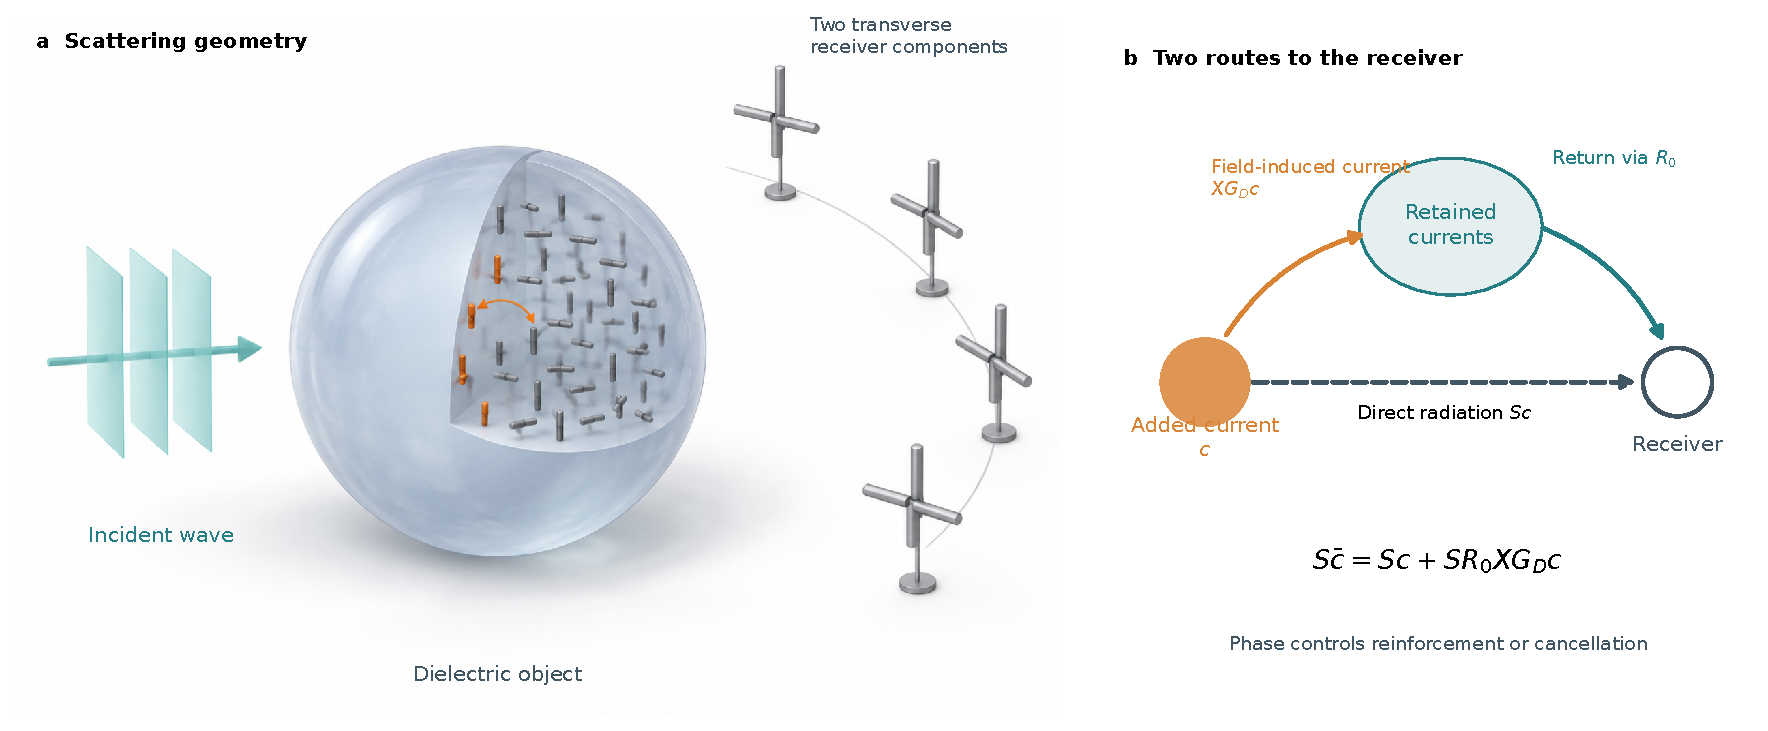
\includegraphics[width=\linewidth]{figures/physical_feedback.pdf}
\caption{新增电流存在两条到达接收器的路径：直接辐射，以及经过保留电流的内部反馈。物体和天线为概念示意，不代表某次计算的场分布。}
\end{figure}

这一点对弱辐射电流尤其重要。即使一个方向的直接接收输出很小，若允许的材料变化能激发它，并且它能经内部耦合返回接收通道，材料导数仍可能受到明显影响。因此，“直接看不见”与“对材料更新无影响”并不是同一件事。


\section{把指定电流改动追到材料这一步}
我用共享的实材料向量$s$表示复介电材料的实部和虚部。材料方向先按体积加权的物理内积正交化，所有illumination共享同一个$s$；场和电流仍为复数。材料切向与接收响应满足
\[
 L\delta j_p=B_ps,\qquad \delta y_p=S\delta j_p,
 \qquad J_p=SL^{-1}B_p.
\]
$B_p$是material injection，包含当前total field和材料响应导数；$L^{-1}$是内部耦合后的响应；$S$把电流送到receiver。DDA使用polarizability $a(\chi)$，因此注入保留$a'(\chi)E_p^{\rm tot}$，而不是把$a$直接当contrast。

设原current basis为$V$，$R_0=V(V^*LV)^{-1}V^*$。新增方向$C$及其诱发的retained response为
\[
 \bar C=(I-R_0L)C=C+R_0XG_DC.
\]
第二项依次经过internal field、material response与retained-space solve。Receiver看到$S\bar C$，而不只是$SC$。指定增广的材料导数差为
\[
 D_C=Y_C\Gamma_C^{-1}N_C,
\]
其中$Y_C=S\bar C$描述反馈后输出，$N_C=C^*(I-LR_0)B$描述材料注入，$\Gamma_C=C^*L\bar C$保留新增方向经原空间返回的耦合。这是包含相位和候选间干涉的整体关系，不能当作三个互不相关的单列权重。

三组构造的自由空间Maxwell见证，直接receiver output低于$1.7\times10^{-16}$，反馈后output norm为0.0672--0.0888，材料导数差达到完整Jacobian的3.56\%--5.22\%。它们说明directly dark currents可以通过内部返回路径影响材料；构造见证不表示任意物体中此现象的频率。

实化以后，指定step difference落在观测与注入两组material pullbacks组成的空间中：
\[
 s_C-s_0\in\operatorname{Range}
 H_0^{-1}[J_0^TY_C,N_C^T].
\]
这个paired closure回答模型改动会影响哪些方向，却不保证这些方向最能修正完整目标的误差。已有数值证据让我保留了这一分别。

\begin{center}\small
\begin{tabularx}{\linewidth}{@{}p{.39\linewidth}X@{}}\toprule
比较的问题&结果与我的理解\\\midrule
Paired repair与specified direct enlargement&平滑72/72、尖锐36/36更好，支持两侧material作用。\\
Equal-rank material Krylov与paired repair&全部72/72、36/36更好；step-change support不是最佳error correction。\\
Paid paired warm start与普通PCG&总时间1.416倍，full-wave RHS 66变342，未获加速。\\
Current-derived inverse的八次复用&已有history时六对象成本比0.773--0.877；cached Ritz在两个对象更快，专门获取history后六对象都失去时间优势。\\\bottomrule
\end{tabularx}
\end{center}

固定current dimension的更广检验也有明确边界。43个无噪声状态、15个对象中，合法current search相对receiver的对象中位完整二次风险比为0.4242，而受测finite-gain规则总体为1.0947。高预算时其绝对风险停在约$10^{-4}$，receiver下降更快；不是分母达到数值底噪。Finite/first-order旧比值0.1171还包含位移和末端swap差别，不能单独归因为曲率项。

这里的full-GN fidelity是当前完整quadratic的步差；精确参考时风险为$\|s-s_*\|_H^2/2$。它不等于final reconstruction error。四个尖锐目标的最终材料误差仍为0.755、0.750、0.560、0.906。独立vector Mie核对在中等对比球的最细$32^3$网格给出复场误差0.252\%、uniform material derivative误差0.731\%；粗高对比球仍有21.40\%误差。这些物理与恢复边界没有被新的frozen-state交换结果替代。

\section{我把选模问题收缩到一个更具体的改动}
陈教授，我从Gaussian/N-Port压缩开始关心这个问题，最初想的是把场和电流算得更省。读SOM、Twofold SOM和S-DBIM以后，我意识到接收可见性、内部传播以及材料一致性已经有很成熟的研究。我的问题逐渐变成：在这些current subspace的基础上，一个指定的current change究竟怎样改变当前material update？

retained feedback给出了其中的物理过程。新增电流既直接辐射，又通过内部场激发原有电流；接收端看到二者的复振幅叠加。反过来，材料变化也可能先进入保留电流，再传到新增方向。这个frequency-domain feedback来自方程消元，不是给某个模式拟合一个经验权重。

我现在把模型改变同时写到data curvature和normal-equation offset里：
\[
 \mathsf I_U=J_U^TJ_U,\qquad h_U=J_U^Tr+\ell,
 \qquad H_Us_U=-h_U.
\]
前者描述材料变化会产生哪些接收响应；后者保留这些响应与当前residual的方向和符号。电流变化产生 $D$ 后，两者分别改变为
\[
 \Delta\mathsf I=J_o^TD+D^TJ_o+D^TD,
 \qquad\Delta h=D^Tr.
\]
因此实际material step difference是
\[
 d=-H_n^{-1}(\Delta h+\Delta\mathsf I s_o).
\]
这也解释了为什么一个transfer norm或information spectrum不足以直接决定选模。相同的 $J^TJ$ 甚至可以对应相反的 $J^Tr$，生成相反的材料步。

为了把这一点检验得更明确，我从receiver spectral backbone出发，只允许少量current exchange。每次动作保持实际current dimension和完整目标不变，用richer reduced anchor提出候选，再用full directional output检查actual finite gain。接受以后重新计算条件邻域，避免用初始评分解释后续所有动作。

我的判断分成三个问题：receiver附近是否确实有更好的current space；有限信息的proposal能找到多少；取得和检查这些信息需要付出多少成本。full-GN fidelity、一次材料真值诊断和最终nonlinear reconstruction分别报告。这里的信息谱作为解释，不替代signed gain，也不把double-precision check称为严格certificate。

\section{Receiver附近确有收益，但找到它的费用也很具体}
四个对象的十二个状态、36个state--budget单元均完成，实际共享current dimension为4、8、16。定向完整复核后的exchange在35个单元有可分辨的完整GN改善，一个单元不变。四对象的汇总风险比中位数为0.348，即完整GN差距下降约65.2\%。这给出了一个明确的正面设计结果：可靠receiver基底只需少量材料相关替换，就能显著改善这一步。对象内先把九个单元的风险相加，再与同一对象的receiver基底比较：
\begin{center}\small\begin{tabular}{@{}lrrr@{}}\toprule
几何 / 材料空间&Local teacher&Verified exchange&Teacher改善取得比例\\\midrule
平滑 / Gaussian&0.0984&0.1904&89.8\%\\
近接触 / Gaussian&0.2016&0.6538&43.4\%\\
分层 / voxel&0.1520&0.2776&85.2\%\\
非对称 / voxel&0.1628&0.4181&69.5\%\\\bottomrule
\end{tabular}\end{center}
前两列是风险比，越小越好。最后一列比较两条最多三个动作的路径各自取得的risk reduction，不是同一checkpoint上的纯评分准确率。Teacher仍须枚举完整声明邻域并支付标签费用。

在每个对象的九个共同receiver checkpoint上，先把单次gain求和再相除，可以更清楚地拆开损失。完整字典anchor top-one的对象级捕获率为98.1--99.6\%，不是每个checkpoint的下界；但十二incoming shortpool只覆盖近接触对象35.3\%的机会，非对称对象65.9\%，平滑和分层对象分别96.9\%、92.0\%。因此，至少在这个共同checkpoint上，近接触对象首先受限于候选覆盖，而不是完整字典内的anchor排名。我没有把不同路径的终点差统统叫作surrogate error。

\begin{figure}[htbp]\centering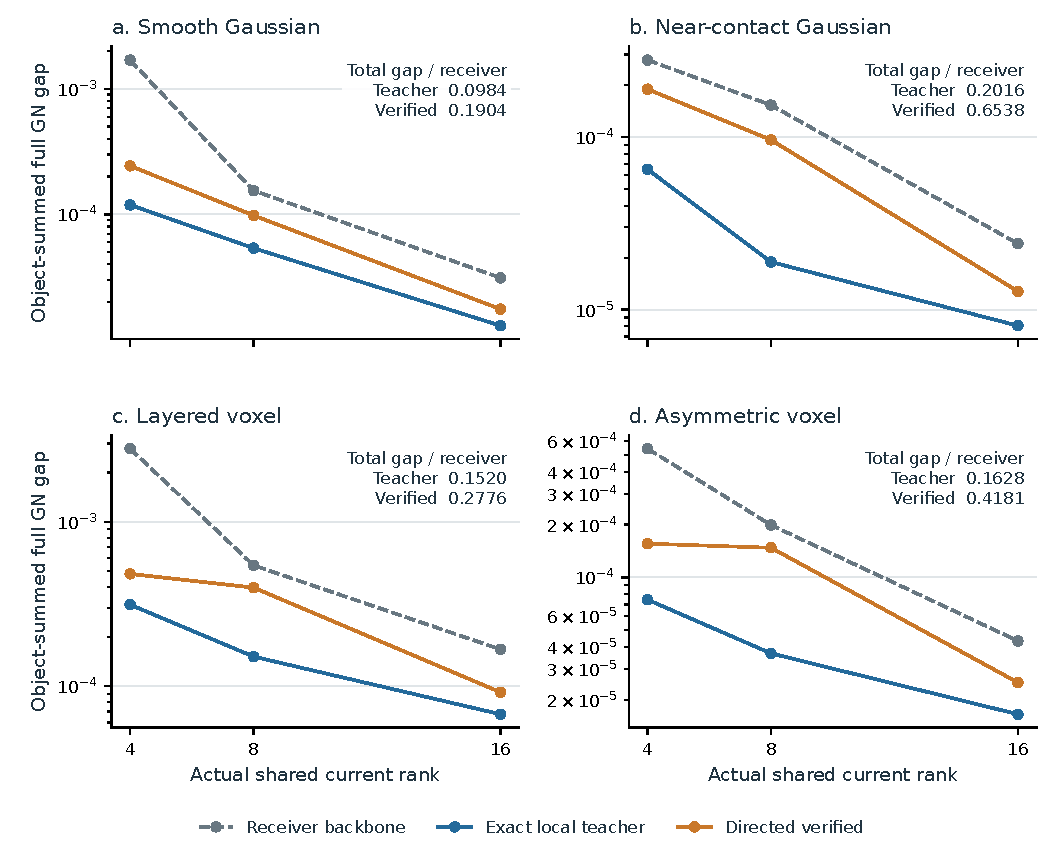
\includegraphics[width=\linewidth]{figures/exchange_risk.pdf}
\caption{三个状态的absolute full-GN gap按对象、current budget汇总。Current teacher只代表声明的局部exchange域；曲线不表示新的nonlinear reconstruction。}
\end{figure}

\section{信息量增加，仍可能把材料步推向错误方向}
我在同一物理材料度量下，将data curvature $\mathsf I_U=J_U^TJ_U$与prior/LM分开。用固定$P=10^{-5}I$归一化后，记录information volume、effective dimension和相对完整曲率的fidelity；voxel仅在十六个共同方向上记录projected diagnostics。这些是固定数值尺度下的局部诊断，没有实测noise covariance支持的互信息解释。

一个近接触对象初始状态的实际交换，使log-det information volume增加6.3127、effective dimension增加1.8613，完整curvature fidelity也略有改善，但actual full gain为$-5.5754\times10^{-5}$。也就是说，一个模型可以声称更多信息，甚至略微改善某个曲率误差指标，却把当前材料步推得更差。这个见证说明information magnitude和该curvature fidelity指标仍不足以决定收益；实际步由residual相关的offset与曲率改变共同决定。这是我认为最需要讲清楚的区别。

另一组common-core测试给出了真实Maxwell相互作用：从rank14开始，分别加一个方向时gain为$-3.2391\times10^{-8}$、$-5.8389\times10^{-8}$，一起加到rank16时变成$3.4787\times10^{-7}$。我将它称为pair interaction witness；它不表示所有greedy方法失效，也不是同秩1-swap局部陷阱。

\section{怎样把这个设计付诸计算，以及接下来需要什么证据}
相同CUDA FP64算子的五次轮换计时中，三个动作上限的conditional selector在近接触Gaussian上为0.594--2.690秒，在分层voxel上为0.891--3.400秒。相同初始shortpool只做一次定向决定为0.328--0.937秒、0.333--1.215秒。公共physical setup与历史anchor/pool acquisition单独计费；这些warm时间没有证明冷启动加速。Receiver不动最便宜；exchange付费换取的是frozen step fidelity。

我也完成了冻结架构的小网络priority pilot，使用对象分组：两个对象训练，一个validation，一个heldout test。MLP的test top-two capture为98.85--99.16\%，group-mean为75.99--98.03\%，都低于已有anchor top-two的99.885\%。特征仍要取得child/anchor信息，fresh physical validation和all-in cost saving没有测得，因此不把这个小试验作为神经选模贡献。

高保真交换检查共接受75个动作，终态22次为信息未解决的abstention、14次达到动作预算。没有合法output-error bound，所以没有严格的acceptance/全邻域停止certificate。允许$\le k$的策略最终仍全部用满$k$，没有取得terminal rank saving。

所有结果首先是full-GN fidelity。无约束$\alpha=1$的一步truth diagnostic相对当前材料，19个单元误差下降、17个上升，28步违反材料约束；它不是line search接受后的重建。Gaussian完整参考在固定prior threshold下也没有full-weak方向；voxel的投影不能断言整个材料空间不弱。我没有据此启动Flow或新的nonlinear reconstruction。

我因此把主线保留为mechanism与conditional local design：材料进入、内部反馈、接收返回共同决定一个模型改动怎样作用；实际是否值得改，还要看offset、curvature、候选覆盖和验证费用。更便宜地识别有用incoming directions，以及把局部gain转成有约束的非线性恢复，仍是最值得进一步弄清楚的部分。

\section{我想进一步请教的物理问题}
我目前最想弄清楚的是，在有限孔径、非均匀材料的真实散射中，怎样用可计算的量判断“材料能激发，而且反馈后能被接收”的方向。现在的分解给出了这两个环节，但把它们压缩成稳定、便宜的选模规则仍有难点。

我也希望结合您对 SOM、TSOM 和 S-DBIM 的理解，讨论这种材料切向视角与原有电流子空间物理的联系：哪些解释只是已有认识的另一种表述，哪些条件确实补充了对材料更新的理解？特别是，若直接辐射很弱而内部返回路径明显，最合适的解释应当从观测孔径、内部传播，还是二者与材料激励的联合结构出发？

最后是计算上的问题。伴随电流样本（adjoint current snapshots）提供了一种把接收信息带回电流空间的方式，但并非在所有状态都值得保留。我想听听您对后续验证重点的建议：怎样选择一个最有辨别力的电磁场景，使不同机制给出可区分、可证伪的预测，而不是继续增加许多相似的性能对照。对选模而言，我特别想找到一个便宜的内部返回量，提前排除许多最后被完整定向检查拒绝的候选。
\section*{主要参考文献与阅读线索}
陈教授的专著\emph{Computational Methods for Electromagnetic Inverse Scattering}（2018）提供逆散射与子空间方法的背景；Chen、Zhong 与 Agarwal（2010）的综述，以及 Zhong 与 Chen（2011）的 FFT-TSOM 工作说明内部传播和外部观测的联合组织；Ye 与 Chen（2017）的 S-DBIM 说明背景场更新与材料求解的联系。de Sturler 等的 插值逆向降阶模型（interpolatory inverse ROM）工作提供正向/伴随包含与导数保持的对照；Gaul 等关于 增广/消去 Krylov（augmented/deflated Krylov）的框架用于标准材料复用比较。完整文献条目见随附英文论文。
\end{document}
